\documentclass[letterpaper,12pt]{article}

% \usepackage[margin=1in]{geometry}
\usepackage{geometry}
% \usepackage{lipsum}
%
% \usepackage{hyperref}
%
\usepackage{graphicx}
\graphicspath{ {images/} }
\synctex=1


% \bibliographystyle{IEEEtran}

\usepackage[utf8x]{inputenc}
\usepackage{float}

\title{ECE 321: Software Requirements Engineering \\ Assignment 3}
\author{Arun Woosaree \\ \\ XXXXXXX}

\begin{document}
\maketitle
% \newpage

\section{}
\begin{figure}[H]
 \centering
 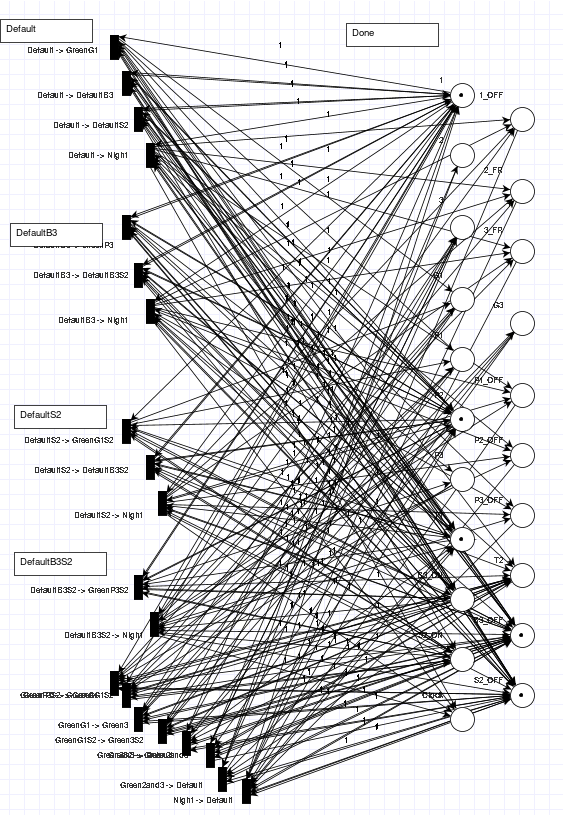
\includegraphics[width=\textwidth]{petrinet.png}
 \caption{Screenshot of the petri net created in PIPE}
 % \label{q6}
\end{figure}

\begin{figure}[H]
 \centering
 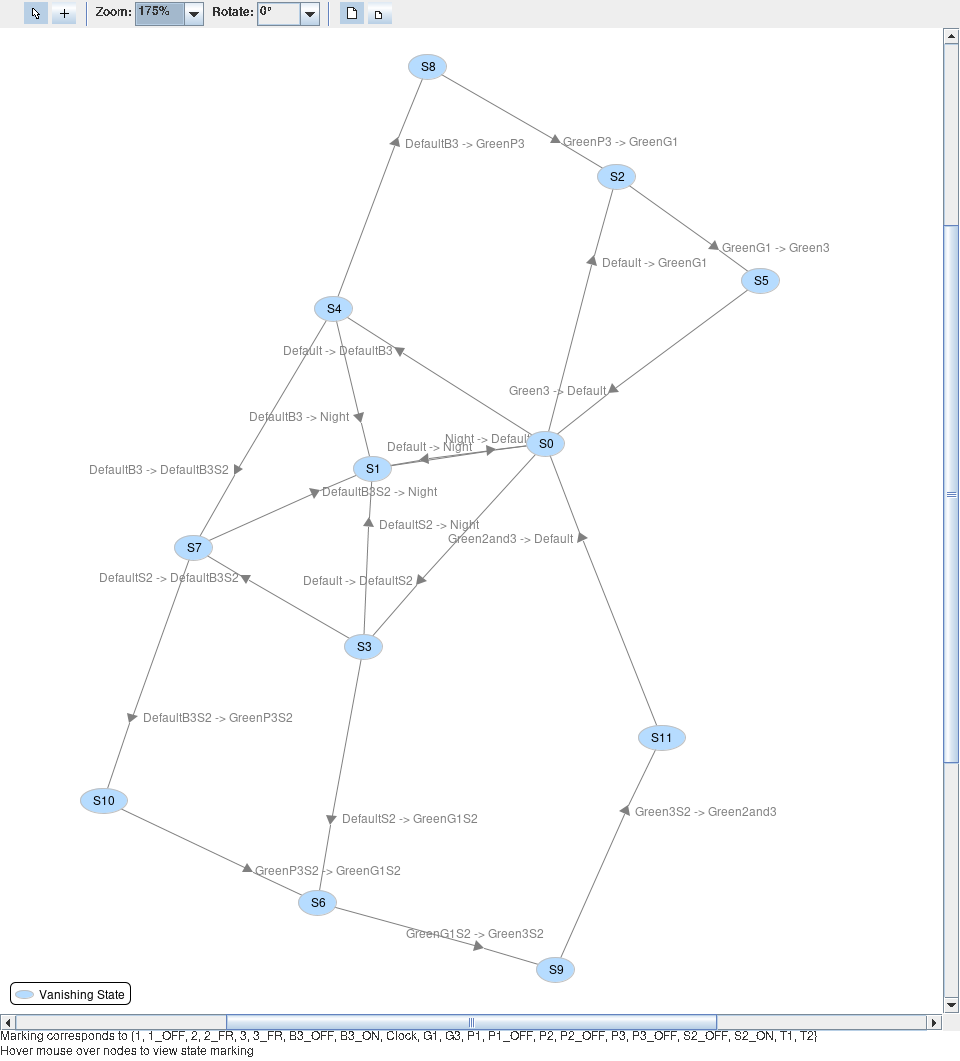
\includegraphics[width=\textwidth]{reachabilitygraph.png}
 \caption{Screenshot of the reachability graph generated from the petri net}
 % \label{q6}
\end{figure}


\section{Description of transitions}
\begin{enumerate}
 \item Default $\rightarrow$ GreenG1
 \item Default $\rightarrow$ DefaultB3
 \item Default $\rightarrow$ DefaultS2
 \item Default $\rightarrow$ Night
 \item DefaultB3 $\rightarrow$ GreenP3
 \item DefaultB3 $\rightarrow$ DefaultB3S2
 \item DefaultB3 $\rightarrow$ Night
 \item DefaultS2 $\rightarrow$ GreenG1S2
 \item DefaultS2 $\rightarrow$ DefaultB3S2
 \item DefaultS2 $\rightarrow$ Night
 \item DefaultB3S2 $\rightarrow$ GreenP3S2
 \item DefaultB3S2 $\rightarrow$ Night
 \item GreenP3 $\rightarrow$ GreenG1
 \item GreenP3S2 $\rightarrow$ GreenG1S2
 \item GreenG1 $\rightarrow$ Green3
 \item GreenG1S2 $\rightarrow$ Green3S2
 \item Green3 $\rightarrow$ Default
 \item Green3S2 $\rightarrow$ Green2and3
 \item Green2and3 $\rightarrow$ Default
 \item Night $\rightarrow$ Default

\end{enumerate}
\section{}

\subsection{Is the model conservative?}

\subsection{Can we have deadlock?}
Using the \textit{Space analysis tool} in PIPE, we see that the model is bounded, safe, and has no deadlock.

\subsection{Can we have starvation?}



\end{document}
